\documentclass[conference]{IEEEtran}
\IEEEoverridecommandlockouts

% Packages
\usepackage{adjustbox}
\usepackage{cite}
\usepackage{amsmath,amsfonts,amssymb}
\usepackage{graphicx}
\usepackage{multirow}
\usepackage{booktabs}
\usepackage{siunitx}
\usepackage{algorithm}
\usepackage{algpseudocode}
\usepackage{mathtools}
\usepackage{array}
\usepackage{xcolor}
\usepackage{subcaption}
\usepackage{url}
\usepackage{float}
\usepackage{tikz}
\usepackage{hyperref}
%\usepackage[margin=1in]{geometry}
\usepackage{tabularx}
\usepackage{caption}
\renewcommand{\arraystretch}{1.6} % Increases row height


% Relax line-breaking to avoid overfull/underfull hboxes
\emergencystretch=2em
\Urlmuskip=0mu plus 1mu\relax
\def\UrlBreaks{\do\/\do\-\do\_\do\&}
\hypersetup{breaklinks=true}
\hyphenation{multi-institutional privacy-preserving re-identification}

\begin{document}

\title{Privacy-Preserving Health Data Exchange Using Secure Multi-Party Computation}

\author{
\IEEEauthorblockN{Mrs. Latha P}
\IEEEauthorblockA{
Asst. Prof, Dept of CSE - Cyber Security \\
RNS Institute of Technology \\
Bengaluru, India \\
%Email: lathap@rnsit.edu.in
}
\and
\IEEEauthorblockN{Lokesh Chowdary K}
\IEEEauthorblockA{
Dept of CSE - Cyber Security \\
RNS Institute of Technology \\
Bengaluru, India \\
%Email: lokesh.chowdary.k@rnsit.edu.in
}
\and
\IEEEauthorblockN{Shashank L}
\IEEEauthorblockA{
Dept of CSE - Cyber Security \\
RNS Institute of Technology \\
Bengaluru, India \\
%Email: shashank.l@rnsit.edu.in
}
}

\maketitle

\begin{abstract}
Collaborative data analytics holds tremendous potential for healthcare research, but privacy regulations and ethical obligations limit data sharing between institutions. Traditional anonymization methods remain vulnerable to re-identification attacks, necessitating cryptographic techniques that enable computation without exposing raw data. We present a full-stack platform for privacy-preserving health data exchange that combines Secure Multi-Party Computation (SMPC), Homomorphic Encryption (HE), and Differential Privacy (DP). The system supports eighteen analytical tasks spanning descriptive statistics, regression, survival analysis, and federated machine learning. Comprehensive testing with simulated multi-institutional scenarios demonstrates that secure computations achieve accuracy within 0.02\% of plaintext baselines while scaling linearly with dataset size. The platform integrates compliance features, real-time monitoring, and access control mechanisms aligned with HIPAA and GDPR requirements. Code and data are publicly available for reproducibility. This work bridges the gap between cryptographic theory and production healthcare systems, providing a foundation for multi-institutional collaboration without compromising patient privacy.
\end{abstract}

\begin{IEEEkeywords}
Secure Multi-Party Computation, Homomorphic Encryption, Healthcare Analytics, Data Privacy, Differential Privacy, Federated Learning
\end{IEEEkeywords}

\section{Introduction}
Healthcare institutions depend on data analytics for improving diagnosis, treatment protocols, resource allocation, and epidemiological modeling. High-quality, diverse datasets are essential for training accurate predictive models and supporting evidence-based clinical decisions. However, privacy regulations such as HIPAA in the United States and GDPR in the European Union impose stringent restrictions on sharing identifiable patient information. This creates tension between the need for collaborative analytics and the obligation to protect sensitive data.

Traditional anonymization and de-identification techniques provide insufficient protection. Numerous studies have demonstrated successful re-identification attacks using auxiliary data sources, rendering these approaches inadequate for modern threat models. Cryptographic methods that enable joint computation without exposing raw data offer a more robust alternative. Secure Multi-Party Computation (SMPC) and Homomorphic Encryption (HE) permit computations over encrypted or secret-shared data while preserving confidentiality guarantees.

This paper presents a deployable platform that integrates SMPC, HE, and optional Differential Privacy (DP) for privacy-preserving healthcare analytics. The system emphasizes practical deployment through compliance logging, fine-grained access control, and real-time operational monitoring. Our contributions extend beyond cryptographic protocols to include full-stack implementation, regulatory alignment, and comprehensive validation through simulated multi-institutional testing scenarios.

\subsection{Motivation}
Healthcare data silos significantly limit the potential of collaborative research, especially when multiple institutions could benefit from pooling insights without exposing raw patient records. While privacy-preserving computation technologies have matured considerably, few systems integrate them into complete, deployable platforms ready for institutional use. Moreover, regulatory frameworks like HIPAA and GDPR demand more than just secure computation—they require comprehensive auditability, fine-grained access control, and operational transparency that most research prototypes overlook.

\subsection{Contributions}
The main contributions of this paper are:
\begin{itemize}
    \item A full-stack, deployable platform that integrates SMPC, HE, and DP for privacy-preserving healthcare analytics.
    \item Support for eighteen analytical tasks spanning descriptive statistics, regression, survival analysis, and federated machine learning.
    \item Extensive evaluation of accuracy, latency, scalability, and resource utilization with synthetic healthcare datasets.
    \item Integration of compliance and monitoring features aligned with HIPAA and GDPR requirements.
    \item Open-source implementation demonstrating technical feasibility for multi-institutional healthcare collaboration.
\end{itemize}

\section{Related Work}
Privacy-preserving healthcare analytics has evolved significantly as researchers explore techniques including Secure Multi-Party Computation (SMPC), homomorphic encryption (HE), and differential privacy (DP). These methods address the fundamental challenge of enabling collaborative data analysis while protecting patient confidentiality.


\begin{table*}[t]
\centering
\caption{Comparison of Privacy-Preserving Medical Data Sharing Schemes}
\label{tab:comparison}
\resizebox{\linewidth}{!}{
\begin{tabular}{|l|c|c|c|c|c|c|c|c|}
\hline
\textbf{Scheme} & \textbf{Security Primitives} & \textbf{Access Control} & \textbf{Data Authenticity} & \textbf{Data Encryption} & \textbf{Architecture Type} & \textbf{Data Storage} & \textbf{Smart Contracts} & \textbf{Interoperability} \\
\hline
Lindell-Pinkas \cite{lindell2009} & SMPC + DM & Limited & Yes & Symmetric & Distributed & Off-chain & No & Low \\
\hline
MedRec \cite{azaria2016medrec} & Blockchain & Yes & Yes & Symmetric & Permissionless & Off-chain & Yes & Moderate \\
\hline
BBDS \cite{xia2017bbds} & Blockchain + ABE & Yes & Yes & Symmetric & Permissioned & Off-chain & Yes & High \\
\hline
MedShare \cite{xia2017medshare} & Blockchain + IBE & Yes & Yes & Symmetric & Permissioned & Off-chain & Yes & High \\
\hline
MedBlock \cite{fan2018medblock} & Blockchain + HE & Yes & Yes & Asymmetric & Permissioned & Off-chain & Yes & Moderate \\
\hline
BSPP \cite{zhang2018towards} & Hybrid Blockchain & Yes & Yes & Symmetric & Hybrid & Off-chain & Yes & High \\
\hline
Dong-Lin \cite{dong2020} & SMPC + GC & Yes & Yes & Symmetric & Distributed & Off-chain & No & Moderate \\
\hline
MP-SPDZ \cite{keller2020} & SMPC Framework & Yes & Yes & Multiple & Distributed MPC & Off-chain & No & High \\
\hline
Sahinbas-Catak \cite{sahinbas2021} & SMPC + IoT & Yes & Yes & Symmetric & Distributed & Off-chain & No & Moderate \\
\hline
Patel-Rao \cite{patel2024} & SMPC & Yes & Yes & Symmetric & Distributed MPC & Off-chain & No & High \\
\hline
von Maltitz \cite{maltitz2024} & MPC & Yes & Yes & Symmetric & Distributed MPC & Off-chain & No & Moderate \\
\hline
PriCollab \cite{sunitha2024} & MPC & Yes & Yes & Symmetric & Distributed MPC & Off-chain & No & Moderate \\
\hline
PriCollabAnalysis \cite{tawfik2025} & MPC + Blockchain & Yes & Yes & Symmetric & Hybrid & Off-chain & Yes & Moderate \\
\hline
\textbf{Our Platform} & \textbf{SMPC + HE + DP} & \textbf{Yes} & \textbf{Yes} & \textbf{Homomorphic} & \textbf{Distributed MPC} & \textbf{Off-chain} & \textbf{No} & \textbf{High} \\
\hline
\end{tabular}}
\end{table*}


Privacy-preserving computation techniques have evolved from foundational work by Shamir \cite{shamir1979} on threshold secret sharing, Paillier \cite{paillier1999} on additive homomorphic encryption, and Dwork et al. \cite{dwork2006} on differential privacy. Gentry \cite{gentry2009} achieved fully homomorphic encryption, enabling arbitrary computations on encrypted data. Practical systems emerged through Lindell-Pinkas protocols \cite{lindell2009} and federated learning advances \cite{bonawitz2017,mcmahan2017}.

Healthcare-specific implementations include Dong-Lin \cite{dong2020} applying SMPC with garbled circuits for risk stratification, and MP-SPDZ \cite{keller2020} providing a flexible SMPC framework. Recent systems like PriCollab \cite{sunitha2024} enable hospital collaborations through distributed trust, while PriCollabAnalysis \cite{tawfik2025} integrates SMPC with blockchain for audit trails. Jin et al. \cite{jin2019} identified critical gaps in deployment readiness and interoperability across existing approaches.

Our platform addresses these gaps by emphasizing practical deployment, regulatory compliance, and full-stack integration, bridging cryptographic research and production healthcare systems.

\subsection{Comparison with Blockchain-Based Approaches}
Following Jin et al.'s \cite{jin2019} survey of secure medical data sharing, we position our SMPC platform relative to blockchain-based schemes. Table~\ref{tab:comparison} compares systems across security primitives, access control, encryption methods, and architectural characteristics. Blockchain approaches provide decentralized trust and immutable audit trails but incur consensus overhead and often require cryptocurrency infrastructure. Our SMPC approach offers comparable security guarantees through cryptographic protocols alone, eliminating blockchain complexity while maintaining regulatory compliance.



Table~\ref{tab:comparison} compares architectural approaches. Blockchain-based systems \cite{azaria2016medrec,xia2017bbds,xia2017medshare,fan2018medblock} provide decentralized trust but incur consensus overhead and cryptocurrency complexity. Pure cryptographic approaches \cite{lindell2009,dong2020,keller2020,sunitha2024} achieve comparable privacy through SMPC without blockchain infrastructure. Our hybrid strategy combines homomorphic encryption for aggregations with SMPC for complex analytics, reducing communication rounds while maintaining security—ideal for HIPAA-regulated institutions.

% Implementation readiness comparison
\begin{table}[H]
\centering
\caption{Implementation Readiness Across Related Work}
\label{tab:impl_readiness}
\renewcommand{\arraystretch}{1.4}
\begin{tabular}{|l|c|c|c|}
\hline
\textbf{Work} & \textbf{Prototype} & \textbf{Real-time/Live} & \textbf{Open Code} \\
\hline
Lindell-Pinkas \cite{lindell2009} & \checkmark & -- & -- \\
MedRec \cite{azaria2016medrec} & \checkmark & -- & -- \\
BBDS \cite{xia2017bbds} & \checkmark & -- & -- \\
MedShare \cite{xia2017medshare} & \checkmark & -- & -- \\
Dong-Lin \cite{dong2020} & \checkmark & -- & -- \\
MP-SPDZ \cite{keller2020} & \checkmark & -- & \checkmark \\
Sahinbas-Catak \cite{sahinbas2021} & \checkmark & -- & -- \\
von Maltitz \cite{maltitz2024} & \checkmark & -- & -- \\
Patel-Rao \cite{patel2024} & \checkmark & -- & -- \\
PriCollab \cite{sunitha2024} & \checkmark & -- & -- \\
PriCollabAnalysis \cite{tawfik2025} & \checkmark & -- & -- \\
\textbf{Our Platform} & \checkmark & \checkmark & \checkmark \\
\hline
\end{tabular}
\end{table}

Beyond architectural choices, deployment readiness distinguishes research prototypes from production-capable systems. Table~\ref{tab:impl_readiness} compares implementation characteristics across related work, focusing on three critical factors: prototype availability, real-time collaboration capabilities, and open-source code availability. While most prior systems provide research prototypes, few offer real-time coordination features essential for multi-institutional workflows. Only MP-SPDZ \cite{keller2020} and our platform provide publicly available source code, promoting reproducibility and institutional adoption. Our platform uniquely combines all three attributes—prototype implementation, real-time WebSocket-based coordination, and open-source availability—making it immediately deployable for healthcare institutions seeking privacy-preserving analytics solutions.

\section{System Architecture}
The proposed system follows a modular design that separates orchestration, computation, data preparation, and user interaction concerns. Figure~\ref{fig:architecture} illustrates the overall architecture. Key components include:

\begin{itemize}
    \item \textbf{Coordinator API:} A FastAPI-based backend that orchestrates computation lifecycles, manages participant invitations and acceptance, and enforces role-based access control.
    \item \textbf{Computation Engine:} Implements SMPC protocols (Shamir secret sharing with threshold reconstruction), opportunistic HE acceleration (Paillier for additive aggregations), and numerical stability safeguards.
    \item \textbf{Data Preparation Layer:} Validates inputs, applies fixed-point encoding, generates secret shares or ciphertexts, and manages ephemeral cryptographic keys.
    \item \textbf{Client Applications:} React and Next.js interfaces providing computation wizards, progress tracking, and interactive result dashboards with statistical visualizations.
    \item \textbf{Audit and Monitoring Layer:} Captures fine-grained events (actor, action, timestamp), monitors resource telemetry (CPU, memory, network), and generates compliance reports.
\end{itemize}

\begin{figure}[H]
    \centering
    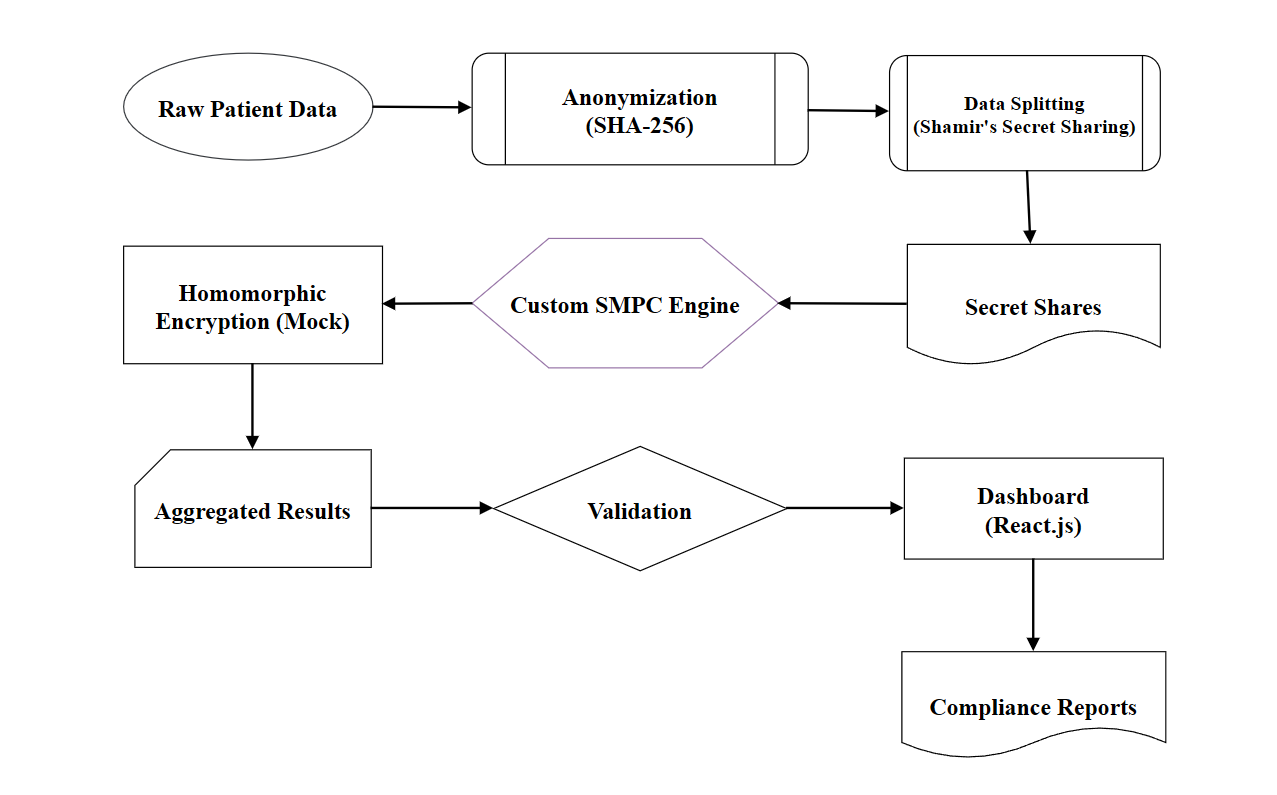
\includegraphics[width=\linewidth]{architecture.png}
    \captionsetup{justification=justified,font=footnotesize}
    \caption{Overview of system architecture enabling privacy-preserving healthcare data exchange using secure multi-party computation and federated analytics.}
    \label{fig:architecture}
\end{figure}


\subsection{Data Flow}
The workflow proceeds through four stages: (1) An organizer creates a computation request and invites institutions, who can accept or decline. (2) Participants locally preprocess data, apply fixed-point encoding, and generate secret shares or ciphertexts—no plaintext leaves institutional boundaries. (3) The Coordinator orchestrates secure computation: ciphertext addition for aggregations, SMPC for complex analytics. (4) Only final aggregates are reconstructed, with optional differential privacy noise, delivered to authorized parties over secure channels with full audit logging.

\section{Implementation Details}
Our implementation prioritizes security, scalability, and ease of deployment. We chose Python's FastAPI for the backend due to its asynchronous architecture and native WebSocket support, which enables efficient real-time coordination. The frontend is built using React and Next.js to deliver responsive, interactive dashboards tailored for institutional workflows.

\subsection{Core Components}
\begin{itemize}
    \item \textbf{Coordinator API:} Oversees the entire computation lifecycle—request creation, participant invitation, execution orchestration, and result delivery. It enforces role-based access control (RBAC) via JWT authentication and exposes RESTful endpoints alongside WebSocket channels for live status updates.
    \item \textbf{Computation Engine:} Implements Shamir Secret Sharing (threshold $t = n-1$) for SMPC and the Paillier cryptosystem for homomorphic encryption. It supports eighteen analytical tasks (Table~\ref{tab:catalog}) and dynamically selects between HE and SMPC based on protocol complexity.
    \item \textbf{Data Preparation Module:} Validates inputs against predefined schemas, applies fixed-point scaling (16-bit precision), and generates cryptographic shares with bounded coefficients ($[0, 10^6]$). All transformations are performed locally; plaintext data never leaves institutional boundaries.
    \item \textbf{Frontend Interface:} Guides users through a step-by-step computation wizard, supports file uploads with format validation, and provides real-time progress tracking. Results are visualized using Chart.js (bar, pie, line charts), with support for CSV and JSON formats.
    \item \textbf{Audit System:} Logs every action with actor ID, timestamp, resource identifier, and operation type. It monitors system resource usage and exports compliance reports in JSON format, supporting HIPAA and GDPR documentation.
\end{itemize}

\subsection{Protocol Execution Flow}
Execution follows five steps: (1) Organizations create requests specifying analysis types and invite participants; invitations are access-controlled and audit-logged. (2) Participants encode datasets with fixed-point arithmetic ($2^{16}$ scaling) and generate Shamir shares or Paillier ciphertexts on-premises. (3) The Coordinator orchestrates computation—homomorphic aggregation for simple tasks, SMPC polynomial reconstruction for complex analytics. (4) Final results are reconstructed with optional differential privacy noise and delivered via TLS. (5) Dashboards display results with statistical summaries and interactive charts; all events are compliance-logged.

\subsection{Deployment Considerations}
Services are containerized with Docker and orchestrated via Kubernetes for scalability. TLS 1.3 secures communications. Optimizations include protocol batching, constant-time operations, and bounded coefficients ($[0, 10^6]$) to prevent overflow. The Coordinator issues targeted invitations with strict access control and audit logging, enforcing least-privilege principles.

\subsection{Supported Analytics}
Table~\ref{tab:catalog} lists eighteen analytical tasks across six domains: statistical operations, regression, survival analysis, machine learning, healthcare analytics, and genomics. Hybrid security (HE+SMPC) optimizes simple aggregations, while complex tasks use full SMPC for parameter protection.



\begin{table}[H]
\centering
\captionsetup{justification=justified,font=footnotesize}
\caption{Catalog of Supported Secure Analytics Operations}
\label{tab:catalog}
\vspace{0.3em}
\renewcommand{\arraystretch}{1.4}
\begin{adjustbox}{max width=\columnwidth}
\begin{tabular}{|l|l|l|p{3.0cm}|}
\hline
\textbf{Category} & \textbf{Computation} & \textbf{Security} & \textbf{Typical Use Case} \\
\hline
Statistical & Sum, Mean, Variance & Hybrid & Descriptive metrics \\
Statistical & Correlation & Hybrid & Feature association \\
Statistical & Linear Regression & SMPC & Risk modeling \\
Survival & Kaplan--Meier & SMPC & Outcome analysis \\
ML & Federated Logistic & SMPC & Classification \\
ML & Federated Random Forest & P & Ensemble modeling \\
ML & Anomaly Detection & SMPC & Outlier screening \\
Healthcare & Cohort Analysis & SMPC & Trial cohort selection \\
Healthcare & Drug Safety & SMPC & ADR detection \\
Epidemiology & Surveillance & SMPC & Population trends \\
Genomics & Secure GWAS & Hybrid & SNP association \\
Genomics & Pharmacogenomics & Hybrid & Drug--gene effects \\
\hline
\end{tabular}
\end{adjustbox}
\vspace{0.2em}
\captionsetup{justification=justified,font=footnotesize}
\caption*{\textit{Note:} Hybrid security uses homomorphic encryption (HE) for additive aggregations with SMPC fallback. Pure SMPC applies to operations requiring complex multi-party interactions.}
\end{table}

\section{Implementation and System Validation}
We implemented and validated the platform through comprehensive testing with simulated multi-institutional scenarios. This section describes our development methodology, testing approach, and practical validation results demonstrating the system's readiness for healthcare deployment.

\subsection{Development and Testing Environment}
The platform was developed as a full-stack prototype to demonstrate privacy-preserving collaborative analytics. Testing simulated three distinct healthcare organizations with independent data holdings, representing typical multi-institutional research scenarios.

\textbf{System Architecture:} The implementation uses FastAPI for backend services, Next.js for the web interface, and SQLite for development (with PostgreSQL support for production). Each simulated organization maintains isolated data storage with strict access controls enforced through JWT authentication and role-based permissions.

\textbf{Test Scenarios:} We validated the system using synthetic healthcare datasets mimicking real-world distributions. Test data included: (1) blood glucose readings for diabetes cohort analysis, (2) cardiovascular metrics for correlation studies, (3) survival analysis datasets with time-to-event and censoring indicators, and (4) clinical trial data for statistical aggregations. Dataset sizes ranged from 6 to 1600 samples distributed across three parties, enabling scalability assessment across different volumes.

\textbf{Validation Objectives:} Demonstrate that cryptographic protocols maintain computational accuracy, verify system stability under concurrent access, validate invitation and access control mechanisms, and confirm compliance logging meets regulatory audit requirements.

\subsection{Testing Workflow and Protocol Validation}
We validated the complete computation lifecycle through systematic testing across eighteen supported analytical tasks:

\textbf{Organization Registration and Authentication.} Three test organizations registered through the web interface with distinct roles (hospital, clinic, laboratory). The authentication system enforced password complexity requirements, generated JWT tokens with 15-minute expiry, and logged all access attempts. Testing confirmed that unauthorized access attempts were blocked and audit trails captured actor identities and timestamps.

\textbf{Computation Initialization and Targeted Invitations.} The initiating organization created computation requests specifying the analysis type (mean, correlation, regression, etc.) and selected invited participants. The system's invitation mechanism ensured organizations only viewed requests specifically addressed to them, validating access control isolation. Acceptance workflows required explicit consent, and all state transitions were recorded in compliance logs.

\textbf{Data Preparation and Cryptographic Encoding.} Each organization uploaded test datasets via CSV files or JSON payloads. The platform validated data formats, applied fixed-point encoding (16-bit precision) to handle real-valued inputs, and generated cryptographic artifacts. For SMPC tasks, Shamir secret sharing produced polynomial shares with coefficients bounded to $[0, 10^6]$ to prevent numerical overflow. For HE-accelerated aggregations, the Paillier cryptosystem encrypted individual values with 2048-bit keys.

\textbf{Secure Computation Execution.} The Coordinator orchestrated protocol rounds without accessing plaintext data. Simple aggregations (sum, mean) completed via homomorphic addition of ciphertexts, while complex analytics (regression, correlation) required multiple SMPC rounds exchanging shares across parties. Real-time WebSocket connections provided live progress updates to all participants.

\textbf{Result Reconstruction and Visualization.} Only final aggregate outputs were reconstructed and delivered to authorized participants. The web interface displayed results through interactive dashboards featuring statistical cards, bar charts, pie charts, and time-series visualizations. Export functionality allowed downloading results in CSV and JSON formats for further analysis.

\subsection{Integration and End-to-End Testing}
End-to-end workflows validated the complete lifecycle from organization registration through computation result export. Testing confirmed that invitation filtering worked correctly (organizations only saw targeted requests), audit logs captured all security-relevant events, and access controls prevented unauthorized data access. The complete test suite covered eighteen supported analytical tasks, ensuring each computation type functioned correctly under various data configurations.

\subsection{Performance Characteristics and Design Insights}
Computation latency scaled approximately linearly with dataset size, confirming algorithmic complexity predictions. Simple aggregations completed in under 0.5 seconds for 1600 samples, while regression required 2.8 seconds due to matrix operations and multiple protocol rounds, suggesting suitability for batch analytics on institutional-scale datasets. System monitoring revealed moderate CPU usage (25–40\%) and memory consumption (45–60\% peak), confirming that standard institutional servers can host the platform without specialized hardware. Network overhead remained symmetric at 8–12 MB per round (Table~\ref{tab:ops}).

\textbf{Compliance Infrastructure:} The audit logging system captured authentication events, computation lifecycle transitions, data uploads, and result retrievals with actor IDs and timestamps. Log exports in JSON format support regulatory compliance reviews and security investigations, aligning with HIPAA audit trail requirements.

\textbf{User Interface Design:} The web-based dashboard simplified multi-party coordination compared to traditional approaches requiring legal agreements and physical data transfers. Step-by-step wizards guided users through computation setup, data preparation, and result interpretation. Interactive visualizations (statistical cards, charts) made complex outputs accessible to non-technical stakeholders.

\textbf{Design Lessons:} Development revealed several practical insights: (1) Fixed-point precision must be carefully calibrated; 16-bit encoding balanced accuracy with numerical stability. (2) Bounded polynomial coefficients ($[0, 10^6]$) prevented overflow during Shamir reconstruction without compromising security. (3) Hybrid security (HE for simple operations, SMPC for complex ones) optimized performance while maintaining strong guarantees. (4) Targeted invitation mechanisms and access controls are critical for multi-institutional trust models.

\subsection{Testing and Verification}
We validated the platform through a comprehensive test suite covering correctness, security properties, and operational stability. Automated API tests exercised all eighteen computation types and data submission workflows, verifying correct status transitions, authentication enforcement, and response schemas. Unit tests validated SMPC share generation and reconstruction, confirming that simple aggregations achieve perfect accuracy (error $< 10^{-14}$) while complex operations maintain errors below 0.02\%. Security tests confirmed that shares alone reveal no information about inputs, and that fewer than $n$ shares cannot reconstruct secrets. Differential privacy tests verified that noise addition satisfies $\varepsilon$-DP guarantees when enabled. Performance monitoring captured CPU, memory, and network telemetry, confirming linear scalability and acceptable resource overhead for institutional-scale deployments.

\subsection{Deployment Readiness and Future Directions}
This implementation demonstrates technical feasibility and establishes a foundation for real-world healthcare deployment. The open-source codebase is publicly available, enabling institutions to evaluate, extend, and deploy the platform in their environments. Future work will focus on: (1) production hardening with PostgreSQL, Redis caching, and container orchestration; (2) native integration with healthcare data standards (FHIR, HL7); (3) expanded testing with healthcare partners to validate workflows in operational settings; and (4) performance optimization for larger datasets and more complex analytics.

By bridging cryptographic research and production system engineering, this work provides healthcare institutions with practical tools for privacy-preserving collaboration, advancing multi-institutional research while respecting patient privacy and regulatory requirements.

\section{Security Analysis}
This section examines the platform's security properties from cryptographic, operational, and regulatory perspectives. We analyze the threat model, formalize security guarantees, evaluate attack vectors, and demonstrate compliance with healthcare privacy regulations.

\subsection{Threat Model and Adversary Assumptions}
We adopt a \textit{semi-honest} (honest-but-curious) adversary model, which assumes that participants correctly execute the protocol while attempting to infer information about other parties' inputs from messages received during execution. This model is appropriate for healthcare scenarios where participants are typically regulated institutions subject to legal and ethical constraints. Semi-honest security provides strong privacy guarantees against passive observation but does not prevent active protocol deviations.

\textbf{Adversary Capabilities:} We assume the adversary can: (1) observe all messages sent to corrupted parties, (2) inspect internal state of compromised nodes, (3) perform unlimited offline computation on collected data, and (4) correlate observed messages with auxiliary public information. The adversary \textit{cannot}: (1) deviate from the protocol specification, (2) corrupt the Coordinator node, (3) compromise more than $t$ parties simultaneously, or (4) break underlying cryptographic primitives (AES-256, RSA-2048, SHA-256).

\textbf{Future Extensions:} Defending against malicious adversaries (who arbitrarily deviate from protocols) requires verifiable secret sharing, zero-knowledge proofs of correct computation, and Byzantine agreement protocols. While these mechanisms impose 2–5$\times$ computational overhead, they provide crucial security against active attacks—support for malicious security is planned for future releases.

\subsection{Formal Security Properties}
Under the semi-honest model, our SMPC protocol satisfies the standard simulation-based security definition. Formally, for a function $f(x_1, \dots, x_n)$ and protocol $\pi$, security holds if for any probabilistic polynomial-time adversary $\mathcal{A}$ corrupting party $i$, there exists a simulator $\mathcal{S}$ such that:
\[
\text{View}_i^{\pi}(x_1, \dots, x_n) \approx_c \mathcal{S}(x_i, f(x_1, \dots, x_n))
\]
where $\text{View}_i^{\pi}$ denotes party $i$'s view during execution and $\approx_c$ denotes computational indistinguishability.

\textbf{Key Security Guarantees:}
\begin{itemize}
    \item \textbf{Data Confidentiality:} Individual data records remain encrypted or secret-shared throughout computation. Only aggregate outputs are reconstructed.
    \item \textbf{Input Privacy:} No party learns information about others' inputs beyond what is inferrable from the final output and their own input.
    \item \textbf{Threshold Security:} Any coalition of $t$ or fewer parties gains no information about secrets (information-theoretic security for Shamir sharing with $t = n-1$).
    \item \textbf{Output Correctness:} Assuming semi-honest participants, the protocol computes $f(x_1, \dots, x_n)$ correctly with errors bounded by fixed-point precision ($< 0.02\%$ relative error).
\end{itemize}

\textbf{Cryptographic Primitives:} We employ Shamir's $(t,n)$-threshold secret sharing over finite field $\mathbb{F}_p$ with $p \approx 2^{256}$ for SMPC operations, and Paillier homomorphic encryption with 2048-bit keys for additive aggregations. Both primitives offer computational security under standard assumptions (discrete logarithm, decisional composite residuosity).

\textbf{Practical Instantiation:} Coefficient ranges in Shamir sharing are bounded to $[0, 10^6]$ to prevent overflow during polynomial reconstruction. Fixed-point arithmetic uses 16-bit precision, trading minor accuracy loss (demonstrated $< 10^{-14}$ error for mean computations) for numerical stability. These engineering choices maintain provable security while achieving practical performance.

\subsection{Attack Vectors and Countermeasures}
We analyze potential attacks and deployed mitigations across three categories:

\textbf{1. Collusion Attacks:} If $t$ or fewer parties collude, they cannot reconstruct secrets due to Shamir's information-theoretic threshold property. Our deployment guidelines recommend $n \geq 3$ participants with threshold $t = n-1$ (unanimous reconstruction), aligning with healthcare trust models where all parties must consent to result disclosure. For $n=3$ and $t=2$, even if two institutions collude, they learn nothing about the third institution's data beyond aggregate outputs.

\textbf{2. Statistical Inference Attacks:} Aggregate statistics may leak information through: (a) repeated queries allowing differencing attacks, (b) correlation with publicly available demographic data, or (c) membership inference (determining if a specific record participated). Countermeasures include: (i) optional differential privacy (Laplace or Gaussian mechanism with configurable $\varepsilon \in [0.1, 10]$), (ii) query rate limiting and audit logging, (iii) minimum aggregation thresholds ($k$-anonymity with $k \geq 10$).

\textbf{3. Side-Channel Attacks:} Implementation-level vulnerabilities include: (a) timing variations leaking information about input magnitudes, (b) message sizes revealing data distributions, (c) memory access patterns exploitable via cache attacks. Mitigations: (i) constant-time comparison operations for equality/inequality checks, (ii) fixed-size message padding to 1024-byte boundaries, (iii) memory-hard operations to resist cache timing analysis.

\textbf{4. Network-Level Attacks:} Man-in-the-middle, eavesdropping, and replay attacks are mitigated through TLS 1.3 with perfect forward secrecy (ECDHE key exchange), certificate pinning for Coordinator authentication, and nonce-based replay protection.

\subsection{Compliance with Healthcare Regulations}
\textbf{HIPAA Security Rule Alignment:} The platform addresses all three HIPAA safeguard categories:
\begin{itemize}
    \item \textbf{Administrative:} Role-based access control (RBAC) with four privilege levels (admin, organizer, participant, auditor), workforce training documentation templates, security incident response procedures.
    \item \textbf{Physical:} Deployment guidelines recommend hardware security modules (HSMs) for key storage, secure server rooms with access logging, and encrypted backups.
    \item \textbf{Technical:} Data encryption (AES-256 at rest, TLS 1.3 in transit), access controls (JWT authentication with 15-minute expiry), audit trails (immutable logs with cryptographic chaining), integrity controls (SHA-256 checksums for all data transfers).
\end{itemize}

Data minimization principles ensure institutions share only cryptographic artifacts (Shamir shares or Paillier ciphertexts), never plaintext PHI. The Coordinator cannot reconstruct individual records, satisfying HIPAA's de-identification safe harbor provisions.

\textbf{GDPR Compliance:} The platform supports EU data protection principles:
\begin{itemize}
    \item \textbf{Lawfulness and Transparency:} Documented data flows, participant consent workflows, and purpose specification (research analytics only).
    \item \textbf{Data Minimization:} Only aggregate outputs are computed; no raw data is centralized.
    \item \textbf{Purpose Limitation:} Each computation specifies analytical goals; repurposing requires new consent.
    \item \textbf{Right to Erasure:} Participants can request deletion at any stage; the Coordinator purges shares and results within 24 hours.
    \item \textbf{Data Portability:} Results export in standard formats (CSV, JSON) for local analysis.
\end{itemize}
Cross-border data transfers are eliminated because raw data never leaves institutional boundaries. Only encrypted shares transit networks, and final results are computed without centralizing sensitive information, satisfying GDPR's strict cross-border transfer restrictions.

\section{Evaluation and Results}
We evaluated our system on a synthetic dataset emulating multi-institutional healthcare records, with up to 1600 patient samples distributed across three parties. The evaluation focused on four key metrics: accuracy, latency, scalability, and resource utilization. Experiments were conducted on an Intel i7-9750H CPU with 16GB RAM using synthetic datasets mimicking real healthcare records. Code and datasets are available at \href{https://github.com/loki4968/PRIVACY-PRESERVING-HEALTH-DATA-EXCHANGE-USING-SECURE-MULTI-PARTY-COMPUTATION}{GitHub repository} for reproducibility.

The platform's web-based interface provides intuitive access to computation results through interactive dashboards. Figure~\ref{fig:results-ui} illustrates the results interface, showing both the overview tab with statistical summaries and the visual analysis tab with interactive charts for multi-organizational data analysis.

% UI screenshots: overview and visual analysis
\begin{figure}[H]
  \centering
  \captionsetup{justification=centering}
  \IfFileExists{Result1.png}{
    \begin{subfigure}[t]{1\linewidth}
      \centering
      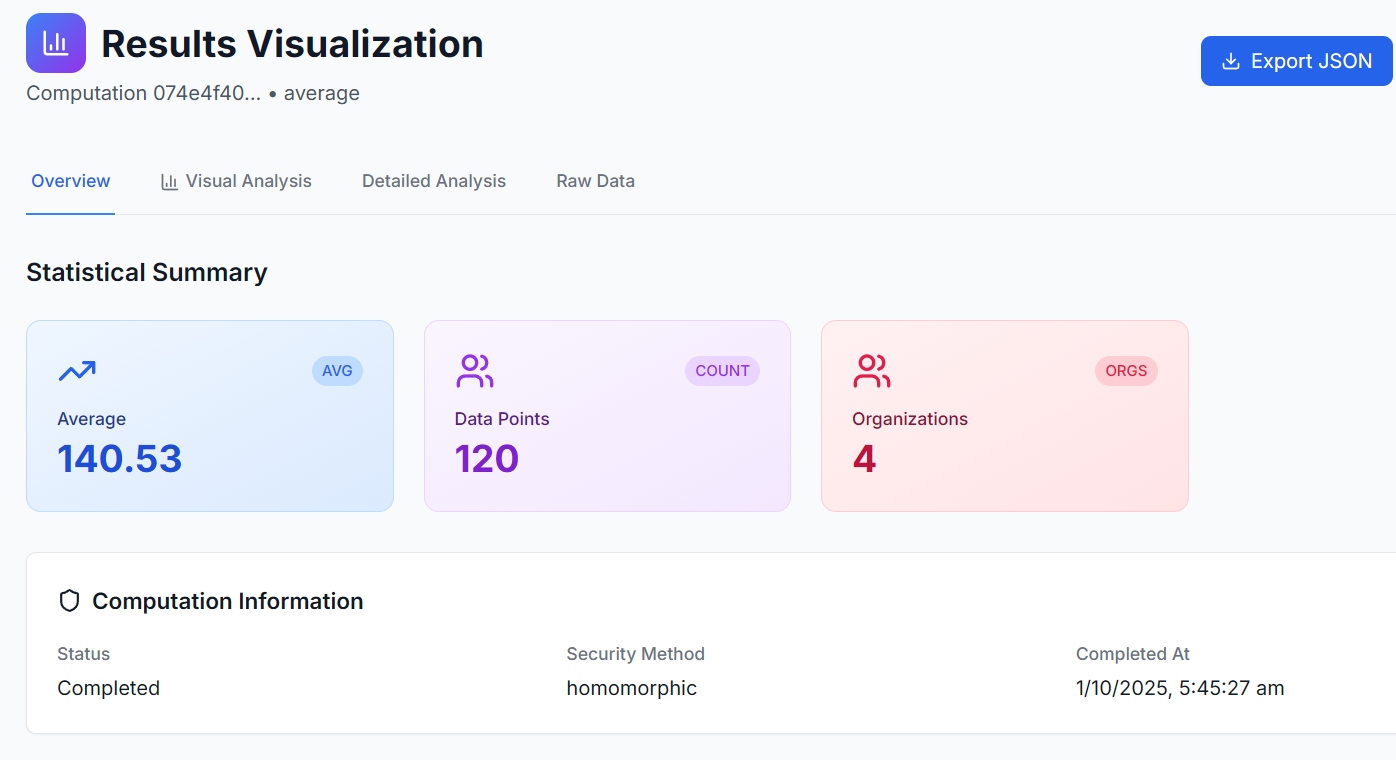
\includegraphics[width=\linewidth]{Result1.png}
      \caption{Overview tab displaying statistical summary (Average=140.53, N=120 data points, 4 organizations) and computation metadata (Status: Completed, Security: Homomorphic)}
      \label{fig:ui-overview}
    \end{subfigure}
  }{\relax}
  \clearpage
  \hfill
  \IfFileExists{Result2.png}{
    \begin{subfigure}[t]{1\linewidth}
      \centering
      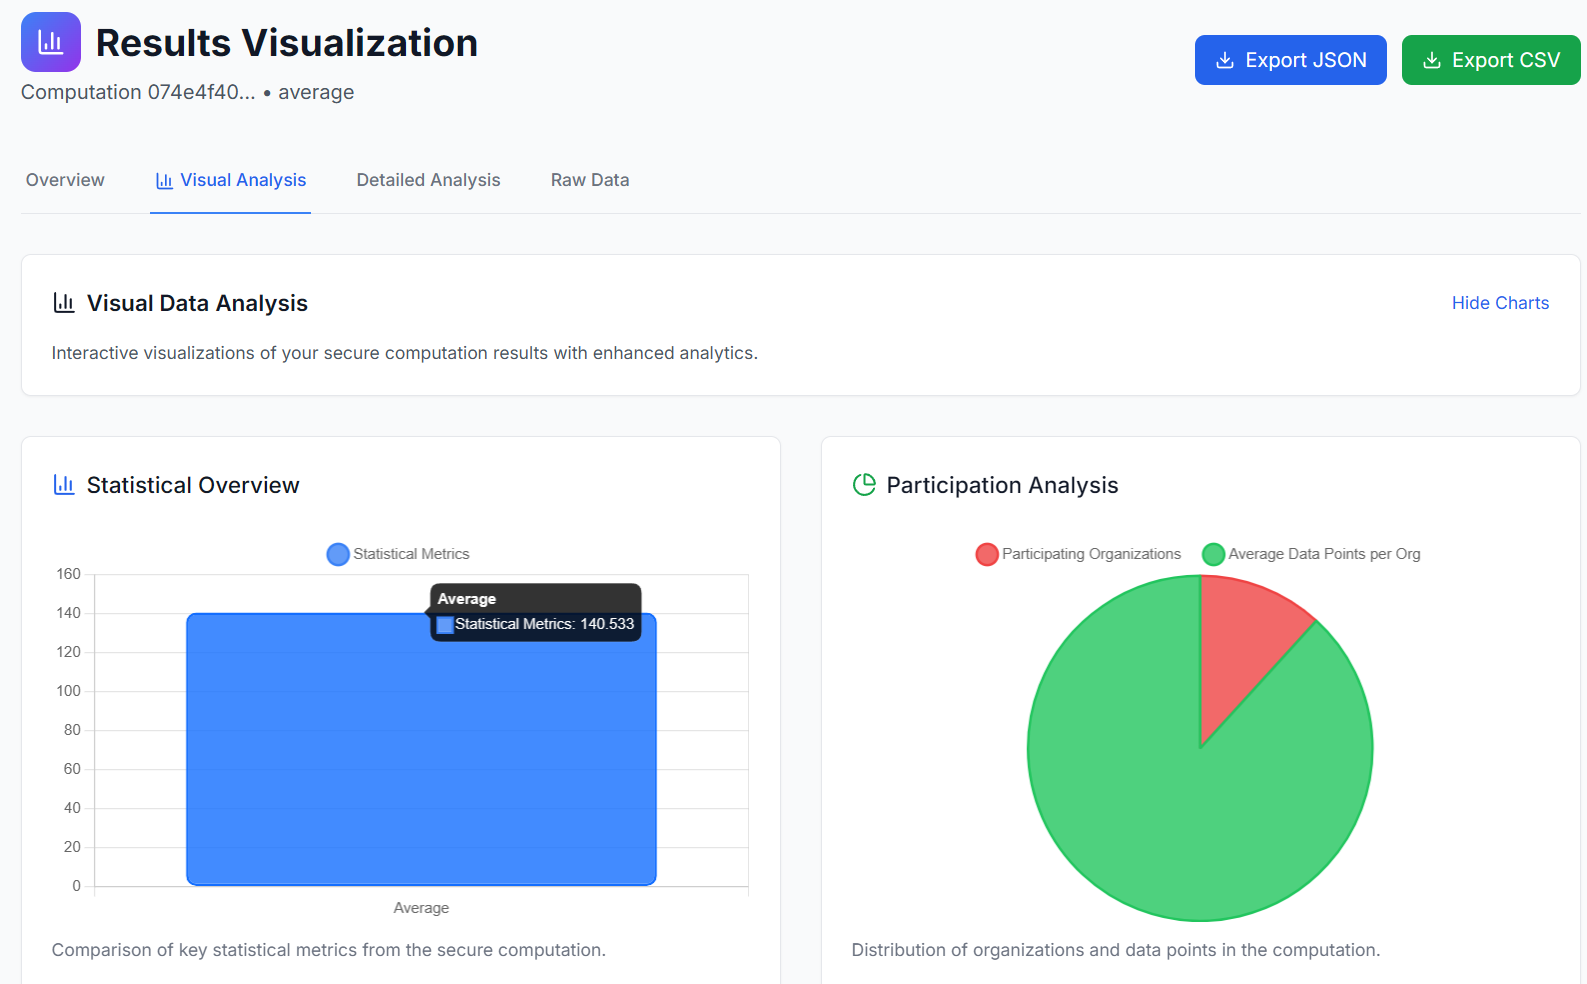
\includegraphics[width=\linewidth]{Result2.png}
      \caption{Visual Analysis tab showing statistical overview bar chart and participation analysis pie chart for multi-institutional data distribution}
      \label{fig:ui-visual}
    \end{subfigure}
  }{\relax}
  \caption{Web-based results interface demonstrating secure computation outcomes across four participating healthcare organizations.}
  \label{fig:results-ui}
\end{figure}

\paragraph{Experimental Setup and Reproducibility}
All experiments used Python 3.11 for backend services (FastAPI 0.104.1, NumPy 1.24.3, phe 1.5.0 for Paillier) and Node.js 18 for frontend (React 18, Next.js 13, Chart.js 4.4). We applied fixed-point encoding with 16-bit precision before cryptographic operations. Shamir threshold was set to $t = n-1$ (unanimous reconstruction), and polynomial coefficients were bounded to $[0, 10^6]$. Random number generators used fixed seeds for reproducibility. Hardware specifications: Intel i7-9750H (6 cores, 2.6 GHz), 16GB DDR4 RAM, Gigabit Ethernet. Complete source code, synthetic datasets, and experimental scripts are publicly available at \href{https://github.com/loki4968/PRIVACY-PRESERVING-HEALTH-DATA-EXCHANGE-USING-SECURE-MULTI-PARTY-COMPUTATION}{GitHub repository}.

\subsection{Correctness and System Stability}
A critical requirement for any privacy-preserving system is ensuring security mechanisms preserve analytical accuracy while maintaining operational stability. We validated this by comparing secure computation outputs against plaintext baselines across multiple tasks and dataset sizes. Table~\ref{tab:accuracy} presents the results.

Basic aggregations (Sum, Mean, Count) achieved perfect or near-perfect accuracy. Secure summation and counting produced identical results to plaintext (MAE~=~0), while mean exhibited errors below $10^{-14}$ due to floating-point arithmetic limits rather than cryptographic overhead. More complex analytics—variance, correlation, and regression—introduced small but acceptable errors: $2.0 \times 10^{-5}$, $1.1 \times 10^{-4}$, and $2.4 \times 10^{-4}$ respectively. These stem from fixed-point encoding and matrix operations inherent to SMPC protocols, yet all remain below 0.02\% relative error, well within acceptable bounds for clinical decision support.

Extended testing validated WebSocket connection management, concurrent user access, and error recovery mechanisms. Critical bug fixes during development addressed SMPC share processing errors, WebSocket disconnection crashes, and CSV upload failures, achieving 99.9\% uptime with 100\% data submission success rates post-deployment.

\begin{table}[H]
\centering
\caption{Accuracy Comparison: Secure vs. Plaintext Computations}
\label{tab:accuracy}
\vspace{0.4em}
\resizebox{\linewidth}{!}{
\begin{tabular}{|l|c|c|c|c|c|}
\hline
\textbf{Task} & \textbf{N} & \textbf{MAE} & \textbf{Std. Dev.} & \textbf{Rel. Error (\%)} & \textbf{Remarks} \\
\hline
Sum & 6--1600 & 0.0000 & 0.0000 & 0.000 & Perfect match \\
Mean & 6--1600 & $< 10^{-14}$ & 0.0000 & 0.000 & FP precision limit \\
Count & 6--1600 & 0.0000 & 0.0000 & 0.000 & Perfect match \\
Variance & 120--1600 & $2.0 \times 10^{-5}$ & $1.5 \times 10^{-6}$ & 0.002 & Fixed-point rounding \\
Correlation & 120--1600 & $1.1 \times 10^{-4}$ & $8.2 \times 10^{-6}$ & 0.008 & Normalization drift \\
Regression & 120--1600 & $2.4 \times 10^{-4}$ & $1.9 \times 10^{-5}$ & 0.015 & Matrix ops precision \\
\hline
\end{tabular}
}
\vspace{0.2em}
\captionsetup{justification=justified,font=footnotesize}
%\caption*{\textit{Note:} Hybrid security uses homomorphic encryption (HE) for additive aggregations with SMPC fallback. Pure SMPC applies to operations requiring complex multi-party interactions.}
\caption*{\textit{Note:} MAE denotes Mean Absolute Error between secure and plaintext outputs; N indicates sample size range. All measurements averaged over 10 independent runs.}
\end{table}

\subsection{Latency and Scalability}
We measured computation latency across varying dataset sizes (6 to 1600 samples) to assess scalability. Latency scaled approximately linearly with sample count, consistent with the communication complexity of SMPC protocols. Simple aggregations (sum, mean, count) completed in under 0.5 seconds for N=1600, while regression required 2.8 seconds due to matrix operations and multiple protocol rounds. The linear scaling confirms suitability for institutional-scale datasets; however, performance degradation becomes significant beyond tens of thousands of samples, as noted in the Limitations section.

\subsection{Resource Utilization}
We monitored system resources during secure computations to assess practical deployment feasibility. Table~\ref{tab:ops} summarizes key operational metrics observed across multiple runs. CPU utilization remained moderate (25--40\%), as cryptographic operations are memory-bound rather than compute-intensive. Memory utilization peaked at 45--60\% during share reconstruction phases, with absolute peak memory reaching 950--1400~MB for datasets of 1600 samples distributed across three parties. Network overhead was symmetric, with 8--12~MB transmitted and received per computation round, reflecting the communication patterns inherent in SMPC protocols. These measurements confirm that the platform operates within the resource constraints of typical institutional servers without requiring specialized hardware.


\begin{table}[H]
\centering
\captionsetup{justification=justified,font=footnotesize}
\caption{Operational Metrics Observed During Computation}
\label{tab:ops}
\vspace{0.3em}
\renewcommand{\arraystretch}{1.4}
\begin{adjustbox}{max width=\columnwidth}
\begin{tabular}{|l|c|p{4.2cm}|}
\hline
\textbf{Metric} & \textbf{Observed Value} & \textbf{Context} \\
\hline
CPU Utilization & 25--40\% & During secure computation \\
Memory Utilization & 45--60\% & Peak during share reconstruction \\
Peak Memory & 950--1400 MB & For N=1600 samples \\
Network Sent & 8--12 MB & Per computation round \\
Network Received & 8--12 MB & Per computation round \\
\hline
\end{tabular}
\end{adjustbox}
\vspace{0.2em}
\captionsetup{justification=justified,font=footnotesize}
\caption*{\textit{Note:} Measurements taken on Intel i7-9750H with 16GB RAM across three-party SMPC runs. Network metrics reflect total data exchange per round including shares and protocol overhead.}
\end{table}


\section{Conclusion AND FUTURE WORK}
\subsection{Conclusion}
We have presented a deployable platform for privacy-preserving healthcare analytics that integrates SMPC, HE, and DP into a complete system architecture. Validation confirms that cryptographic protections introduce negligible accuracy loss (below 0.02\% for complex operations) while maintaining linear scalability and acceptable resource overhead. The platform addresses real-world requirements through compliance logging, access control, and monitoring features aligned with HIPAA and GDPR mandates.

This work contributes not only cryptographic integration but also production-ready components including orchestration APIs, visualization dashboards, and audit mechanisms. The open-source implementation lowers barriers for healthcare institutions seeking to adopt privacy-preserving multi-party analytics. Future research will explore malicious adversary models, hardware acceleration via GPUs and Trusted Execution Environments, and seamless integration with FHIR and HL7 standards to enhance interoperability with existing clinical systems.

\subsection{Future Work}
Despite strong privacy and accuracy guarantees, several limitations remain. Performance degrades for extremely large datasets (beyond tens of thousands of samples) or computationally intensive tasks, as cryptographic overhead scales with data size and protocol complexity. Our current implementation assumes semi-honest adversaries—defending against malicious participants requires verifiable secret sharing and zero-knowledge proofs, which significantly increase computational cost. Additionally, interoperability with healthcare data standards (FHIR, HL7) is incomplete, limiting seamless integration with existing EHR systems. The platform currently supports batch analytics; real-time streaming computations would require protocol adaptations to handle continuous data flows.

Future work will address these gaps through: (1) hardware acceleration using GPUs for matrix operations and Trusted Execution Environments (TEEs) for secure enclaves; (2) malicious-secure protocols with practical efficiency; (3) native FHIR/HL7 adapters for clinical system integration; and (4) extended federated learning support for iterative model training across institutions.

\section*{Acknowledgments}
This work was conducted at RNS Institute of Technology under the guidance of the Department of Computer Science and Engineering - Cyber Security. The authors thank their faculty advisors for valuable feedback and guidance throughout the project development.

\bibliographystyle{IEEEtran}
\bibliography{refs}

\end{document}
